% Figure from MATH 591 notes, section 51. Compile with the notes preamble.
\begin{tikzpicture}[scale=1.15, font=\scriptsize]
\draw[->, gray!55] (-2.6,0) -- (2.7,0) node[right, text=black] {$x$};
\draw[->, gray!55] (0,-2.4) -- (0,2.5) node[above, text=black] {$y$};
\draw[red!70!black, line width=1.4pt] (-2.5,0) -- (0,0);
\node[red!70!black, anchor=south] at (-1.7,0.05) {$\vartheta \to \pi$};
\node[red!70!black, anchor=north] at (-1.7,-0.05) {$\vartheta \to -\pi$};
\draw[->, violet!75!black, thick] (0.573,0.177) -- (0.411,0.703);
\draw[->, violet!75!black, thick] (0.133,0.585) -- (-0.403,0.707);
\draw[->, violet!75!black, thick] (-0.44,0.408) -- (-0.814,0.004);
\draw[->, violet!75!black, thick] (-0.573,-0.177) -- (-0.411,-0.703);
\draw[->, violet!75!black, thick] (-0.133,-0.585) -- (0.403,-0.707);
\draw[->, violet!75!black, thick] (0.44,-0.408) -- (0.814,-0.004);
\draw[->, violet!75!black, thick] (1.29,0.399) -- (1.217,0.632);
\draw[->, violet!75!black, thick] (0.809,1.081) -- (0.613,1.227);
\draw[->, violet!75!black, thick] (0.019,1.35) -- (-0.225,1.353);
\draw[->, violet!75!black, thick] (-0.778,1.103) -- (-0.978,0.962);
\draw[->, violet!75!black, thick] (-1.278,0.435) -- (-1.357,0.204);
\draw[->, violet!75!black, thick] (-1.29,-0.399) -- (-1.217,-0.632);
\draw[->, violet!75!black, thick] (-0.809,-1.081) -- (-0.613,-1.227);
\draw[->, violet!75!black, thick] (-0.019,-1.35) -- (0.225,-1.353);
\draw[->, violet!75!black, thick] (0.778,-1.103) -- (0.978,-0.962);
\draw[->, violet!75!black, thick] (1.278,-0.435) -- (1.357,-0.204);
\draw[->, violet!75!black, thick] (1.958,0.606) -- (1.911,0.76);
\draw[->, violet!75!black, thick] (1.502,1.396) -- (1.392,1.513);
\draw[->, violet!75!black, thick] (0.747,1.909) -- (0.598,1.968);
\draw[->, violet!75!black, thick] (-0.155,2.044) -- (-0.315,2.032);
\draw[->, violet!75!black, thick] (-1.026,1.775) -- (-1.166,1.694);
\draw[->, violet!75!black, thick] (-1.695,1.153) -- (-1.785,1.02);
\draw[->, violet!75!black, thick] (-2.027,0.304) -- (-2.051,0.145);
\draw[->, violet!75!black, thick] (-1.958,-0.606) -- (-1.911,-0.76);
\draw[->, violet!75!black, thick] (-1.502,-1.396) -- (-1.392,-1.513);
\draw[->, violet!75!black, thick] (-0.747,-1.909) -- (-0.598,-1.968);
\draw[->, violet!75!black, thick] (0.155,-2.044) -- (0.315,-2.032);
\draw[->, violet!75!black, thick] (1.026,-1.775) -- (1.166,-1.694);
\draw[->, violet!75!black, thick] (1.695,-1.153) -- (1.785,-1.02);
\draw[->, violet!75!black, thick] (2.027,-0.304) -- (2.051,-0.145);
\draw[teal!60!black, thick, dashed] (0,0) circle (1);
\node[teal!60!black, anchor=west] (C) at (2.35,-1.25) {$c(t) = (\cos t, \sin t)$};
\draw[teal!60!black, thin] (C.west) -- (0.82,-0.57);
\fill[white] (0,0) circle (2.2pt); \draw (0,0) circle (2.2pt);
\node[anchor=north west] at (0.05,-0.05) {hole};
\node[align=center] at (0,-2.85) {$\omega = \dfrac{x\,dy - y\,dx}{x^2 + y^2}$ drawn as arrows (length $1/r$): along every circle;\\ $\omega = d\vartheta$ off the red slit, where the angle $\vartheta$ jumps by $2\pi$};
\end{tikzpicture}
